\chapter{Literature Study}
\label{ch:LiteratureStudy}
%\ifpdf
    \graphicspath{{Chapter2/Chapter2Figures/}}
%\else
    %\graphicspath{{Chapter2/Chapter2Figures/}}
%\fi

In the previous chapter the problem statement and objectives of this project was laid out. Further a brief system overview was also provided.
This chapter will provide information about already existing systems and the techniques they use in doing image processing and character recognition on images. Additionally, research on existing libraries, to aid in this project, will also be done.

\section{Existing systems}
A Optical Mark Recognition(OMR) system is a piece of software that is used to extracted hand written information from a filled in form. Each system normally has a specific template that it can extract information from. An template for one of these forms can be seen in Figure \ref{fig:omrTemplate}. These systems are generally used when fast and accurate grading of tests are needed. The biggest drawback of these systems are that information can only be portrayed in a very limited manner. On OMR templates there are a bubbles that allows a user to chose between different options to answer. OCR systems are thus excellent for the grading multiple choice type questions.At the moment most of these systems only grade colour-in bubbles and do not interpret characters on the page.

\subsection{Standard OMR techniques}
\label{sec:StandardTech}
As can be seen in Figure \ref{fig:omrTemplate}, there is normally specific reference blocks on a OMR template. These blocks are included to allow the computer vision and image processing algorithms find the orientation of the image more easily.

\begin{figure}
  \centering
  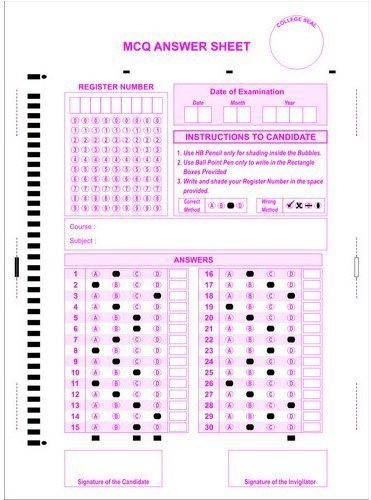
\includegraphics[width=10cm]{omrTemplate}\\
  \caption{Standard OMR template, from \citet{stdTemplate}}%, 
  \label{fig:omrTemplate}
\end{figure}

In an OMR system there are normally two phases to marking an test, as stated in \citet{DraganI2003}. The first step is to determine the region within where the answers are located in the image. In this process the system finds the orientation of the template in the image and thus can approximate the location of the bubbles. Normally some preprocessing on a blank template is done beforehand too aid in locating the bubbles. Once the bubbles are found their locations gets stored and processed. The final step is then to calculate the average pixel concentration in the bubbles and estimate whether they have been filled in.

\section{Additional techniques}
\nomenclature[A]{$OCR$}{Optical character recognition}
The above method allows for grading of tests using a simple OMR system. For the test grader used for the Applied Mathematics tests, there is a need to go beyond such a basic system.  In standard OCR, when a student makes a mistake, he/she needs to erase the existing answer and write a new answer in. This can be time consuming for a template with 8 bubble row choices per answer. This also increases the probability that the student will make a mistake in the process. Addressing this problem it is determined that two additional options need to be made available. Firstly the student is allowed to cross out answers instead of totally erasing them. An example of this can be seen in Figure \ref{fig:Cross}. Then secondly the system needs to be accurate enough to determine the student's student number only by filling in the character blocks above the bubbles. This requirement is addressed by using a PGM in Section \ref{sec:pgmStudentNum}. Using optical character recognition (OCR), the bubble information and character information can thus be cross-referenced in an intelligence way, as seen in Section \ref{sec:PGM}.

\begin{figure}
  \centering
  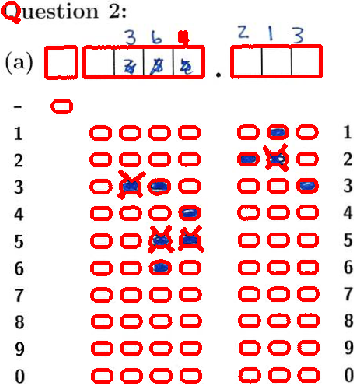
\includegraphics[width=5cm]{Cross}\\
  \caption{Corrected answer by crossing out bubbles.}
  \label{fig:Cross}
\end{figure}

\subsection{Contour detection}
To determine if an answer in a bubble is truly coloured in and not just crossed out, contour detection is needed. This means that the contour around the bubble needs to be detected and used in analysis. In python this can be implemented using the freely available OpenCV library, as referenced in \citet{AdrianR2016}. OpenCV is an image processing library has has highly optimized techniques to find contours in a given image. Given this new contour information the bubbles is can now be assessed by the pixels inside it, as well as its shape. (Verander die image dalk na een wat 'n contour om het)

\subsection{Character recognition}
To further increase the accuracy of the system, Optical Character Recognition (OCR) software will also be need and applied on the characters blocks, present on the templates. Research shows that one preferred way of doing OCR is using TensorFlow. This method is described in \citet{Tensor}. TensorFlow is also a python library, but allows the build of instructions to be implemented in ef{f}icient c++ code. For this test grader, TensorFlow is used to construct a convolutional neural network. This network will read an image, containing the digit, and predict the probability of each digit.

\section{Conclusion: System requirements}

In conclusion it can be seen that the system will need to incorporate a combination of image processing(OMR) on the bubbles and character recognition on the digits, handwritten by the students. When these dif{f}erent evidience is the considered in combination, a more accurate student answer can be estimated. This will also allow for more convenience for students writing these test, hoekom?. Kyk na oom Johan se raad. Die litriture study moet oor huidige metodes gaan en hul resultate.
